\documentclass{article}
\usepackage[utf8]{inputenc}
\usepackage[margin=1.0in]{geometry}
\usepackage{amsmath}
\usepackage{amssymb}
\usepackage{fancyhdr}
\usepackage{physics}
\usepackage{wrapfig}
\usepackage{hyperref}
\usepackage{multirow}
\usepackage{amsthm}
\usepackage{pgfplots}

\pgfplotsset{compat=1.16}



\renewcommand{\thesubsection}{\thesection\Alph{subsection}}
\renewcommand\qedsymbol{\square}



\title{Classical Mechanics PS1}
\author{Joe Crowley}
\date{October 2020}

\pagestyle{fancy}
\renewcommand{\headrulewidth}{0pt}
\renewcommand{\footrulewidth}{1pt}

\fancyhf{}
\rhead{
Joe Crowley \\
Physics 205 \\
Problem Set 2\\
}
\rfoot{Page \thepage}

\begin{document}  

\section{GPS Derivation 2.3}
\textit{Prove that the shortest distance between two points in space is a straight line.}
\begin{proof}
    The length of an infinitesimal arc along the path $ds$ is given by 
    \begin{align*}
        ds &= \sqrt{dx^2 + dy^2} \\ 
        &= \sqrt{1+ \left( \frac{dy}{dx}\right)^2 }dx,
    \end{align*}
    which can be integrated to find the total length of the path. Applying a variation to the length of the curve and setting it stationary yields 
    \begin{align*}
        S &= \int{ds}\\
        \delta S &= \int{\delta \sqrt{1+ \left( \frac{dy}{dx}\right)^2 }dx}\\
        &= \int{\frac{\frac{dy}{dx}} {\sqrt{1+ \left( \frac{dy}{dx}\right)^2 }} \delta \frac{dy}{dx}dx}.
    \end{align*}
    Using the equivalence of mixed partials and integrating by parts, with $u = \frac{\frac{dy}{dx}} {\sqrt{1+ \left( \frac{dy}{dx}\right)^2 }}$ and $dv = \frac{d}{dx}\delta y \,dx$, 
    \begin{align*}
        \delta S&= \int{\frac{\frac{dy}{dx}} {\sqrt{1+ \left( \frac{dy}{dx}\right)^2 }} \frac{d}{dx}\delta y \,dx}\\
        &=-\int{\delta y \,\frac{d}{dx}\left( \frac{\frac{dy}{dx}} {\sqrt{1+ \left( \frac{dy}{dx}\right)^2 }}\right) dx}
    \end{align*}
    This holds true for any $\delta y$, which implies
    \begin{align*}
        \frac{d}{dx}\left( \frac{\frac{dy}{dx}} {\sqrt{1+ \left( \frac{dy}{dx}\right)^2 }}\right) & = 0\\
        \frac{\frac{dy}{dx}} {\sqrt{1+ \left( \frac{dy}{dx}\right)^2 }} &= c_1\\
        \left(\frac{d y}{d x}\right)^{2} &= c_{1}^{2}+c_{1}^{2}\left(\frac{d y}{d x}\right)^{2}\\
        \frac{d y}{d x}&=\sqrt{\frac{c_{1}^{2}}{1-c_{1}^{2}}}\\
        y&=\sqrt{\frac{c_{1}^{2}}{1-c_{1}^{2}}} x+c_{2}.
    \end{align*}
        This is the equation of a line with slope $\sqrt{\frac{c_{1}^{2}}{1-c_{1}^{2}}}$ and intercept $c_2$.
\end{proof}
\newpage 

\section{GPS Exercise 2.5}
\textit{A particle is subjected to the potential $V(x)=-F x,$ where $F$ is a constant. The particle travels from $x=0$ to $x=a$ in a time interval $t_{0}$. Assume the motion of the particle can be expressed in the form $x(t)=A+B t+C t^{2}$. Find the values of $A, B$, and $C$ such that the action is a minimum.}

The Lagrangian for this particle is
\begin{equation*}
    L=\frac{1}{2} m \dot{x}^{2}+F x. 
\end{equation*}

Setting the initial conditions $x(0) = A = 0, x(t_0) = B t_{0}+C t_{0}^{2} = a$ puts constraints on two of the parameters, $A,B$. The action is written as

\begin{align*}
    S &= \int{dt L}\\
     &= \int_{0}^{t_{0}} \frac{1}{2} m(B+2 C t)^{2}+F\left(B t+C t^{2}\right) d t\\
     &= \frac{1}{2} B^2 m t_0+B C m t_0^2+\frac{1}{2} B F t_0^2+\frac{2}{3} C^2 m t_0^3+\frac{1}{3} C F t_0^3\\
     &= \frac{a^{2}}{2} m \frac{1}{t_{0}}+\frac{a F}{2} t_{0}+\frac{C}{6}(C m-F) t_{0}^{3}. 
\end{align*}

To find the stationary point of the action, 
\begin{align}
    \frac{\partial S}{\partial C} &= 0\\
    C &= \frac{F}{2 m }.
\end{align}

Plugging the value of C into the equation $ B=\frac{a-C t_{0}^{2}}{t_{0}}$ gives the parameters $A,B,C$ as
\begin{equation*}
\boxed{
    \begin{array}{l}
        A=0 \\
        B=\frac{\left(a-\frac{F}{2 m} t_{0}^{2}\right)}{t_{0}} \\
        C=\frac{F}{2 m}
    \end{array}
    }
\end{equation*}

\newpage

\section{GPS Exercise 2.13}
\textit{A heavy particle is placed at the top of a vertical hoop. Calculate the reaction of the hoop on the particle by means of the Lagrange's undetermined multipliers and Lagrange's equations. Find the height at which the particle falls off.}

\begin{figure}[h!] 
    \centering
    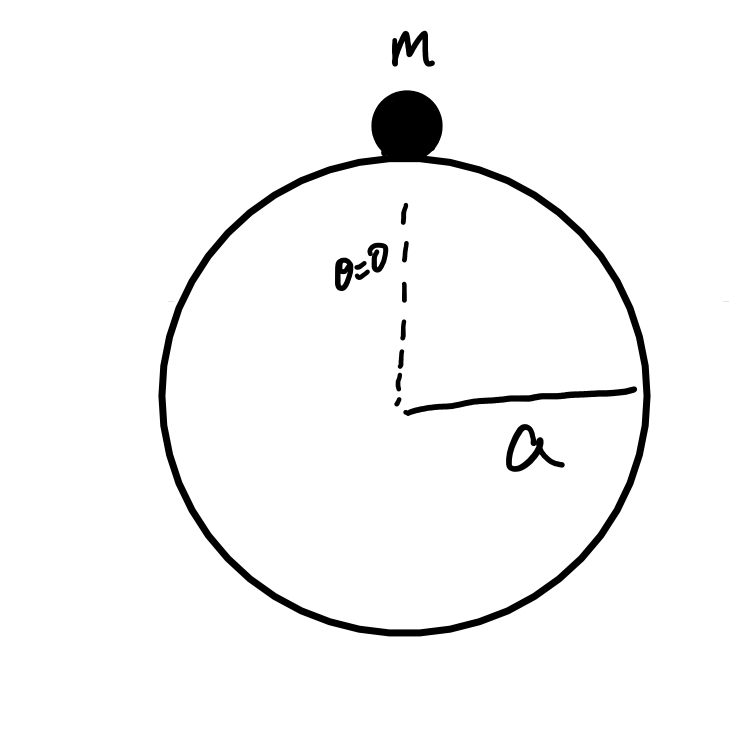
\includegraphics[width=0.3\textwidth]{figures/problem_13.png}
    \label{fig:my_label}
\end{figure}

The Lagrangian for this particle is 
\begin{equation*}
    L = \frac{1}{2}m\left(\dot{r}^2 + r^2 \dot{\theta}^2 \right) - m g r \cos \theta.
\end{equation*}
However, the particle is subject to a constraint $f - r = 0$ while it is still on the hoop. The Euler-Lagrange equation for the radial degree of freedom is 
\begin{align*}
    \frac{d}{d} \frac{\partial L}{\partial \dot r}-\frac{\partial L}{\partial r}+\lambda \frac{\partial f}{\partial r}&=0 \\
    m \ddot{r}-m r \dot{\theta}^{2}+m g \cos \theta+\lambda&=0.
\end{align*}

The Euler-Lagrange equation for the angular degree of freedom is
\begin{align*}
    \frac{d}{d t} \frac{\partial L}{\partial \theta}-\frac{\partial L}{\partial \theta}+\lambda \frac{\partial f}{\partial \theta}&=0\\
    m r^{2} \ddot{\theta}-m g r \sin \theta&=0, \\
\end{align*}
which can be solved for $\dot\theta$ by taking a First Integral:
\begin{align*}
    \ddot{\theta} \dot{\theta}&=\frac{g}{r} \sin \theta \dot{\theta}\\
    \dot{\theta}^{2}&=-\frac{2 g}{r} \cos \theta+c_{1}.
\end{align*}
When $\theta= \dot \theta = 0$, 
\begin{equation*}
    c_1 = \frac{2g}{r}.
\end{equation*}

Plugging $\dot{\theta}^{2}=\frac{2g}{r}(1-\cos \theta)$ back into the EL equation for r, 

\begin{align*}
    m \ddot{r}-m r\left(\frac{2g}{r}\right)(1-\cos \theta)+mg \cos \theta&=\lambda\\
    -2 m y+3 m g \cos \theta&=\lambda.
\end{align*}

The particle falls off the hoop when $\lambda = 0$, which corresponds to an angle $\theta = \arccos\frac{2}{3}$ and a height $h = \frac{2}{3} a$. 
\newpage


\section{GPS Exercise 2.18}
\textit{A point mass is constrained to move on a massless hoop of radius $a$ fixed in a vertical plane that rotates about its vertical symmetry axis with constant angular speed $\omega$. Obtain the Lagrange equations of motion assuming the only external forces arise from gravity. What are the constants of motion? Show that if $\omega$ is greater than a critical value $\omega_{0}$, there can be a solution in which the particle remains stationary on the hoop at a point other than at the bottom, but that if $\omega<\omega_{0}$, the only stationary point for the particle is at the bottom of the hoop. What is the value of $\omega_{0} ?$}

\begin{figure}[h!] 
    \centering
    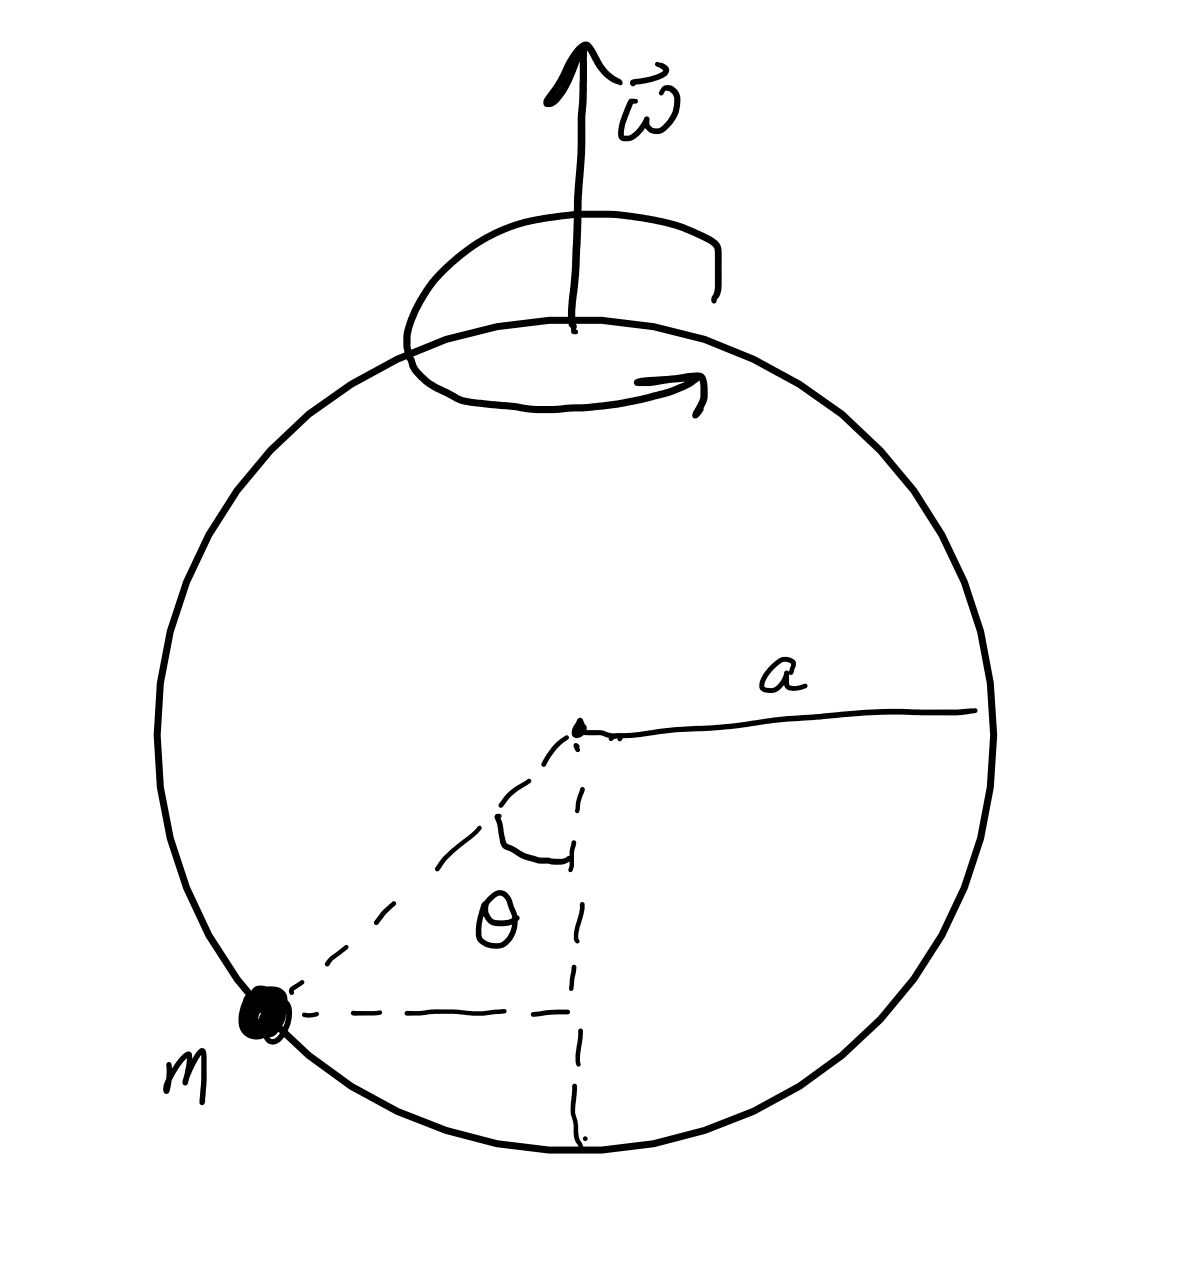
\includegraphics[width=0.3\textwidth]{figures/problem_18.png}
    \label{fig:my_label}
\end{figure}

Note that there is only one degree of freedom, namely the angle $\theta$, measured from the bottom position on the hoop. The Lagrangian for this system is 

\begin{equation*}
    L=\frac{1}{2} m a^{2}\left(\dot{\theta}^{2}+\omega^{2} \sin ^{2} \theta\right)+\operatorname{mg} a \cos \theta.
\end{equation*}

The Euler-Lagrange equation for this system is 

\begin{align*}
    \frac{d}{d t} \frac{\partial L}{\partial \dot\theta}-\frac{\partial L}{\partial \theta}&=0\\
    \operatorname{ma}^{2} \ddot{\theta}-m a^{2} \omega^{2} \sin \theta \cos \theta+\operatorname{mg} a \sin \theta&=0. 
\end{align*}

Solving this equation for $\ddot\theta$, 

\begin{equation*}
    \ddot{\theta}=-\frac{g}{a} \sin \theta+\omega^{2} \sin \theta \cos \theta, 
\end{equation*}
which can be used to determine the frequency $\omega_{0}$. When $\omega > \omega_{0}\, \text{and}\, \theta \neq 0$, 

\begin{equation*}
    \frac{g}{a} \sin \theta=\omega_{0}^{2} \sin \theta \cos \theta.
\end{equation*}
For the particle to have a stable equillibrium at $\theta$, 
\begin{equation*}
    \implies \omega_{0}=\sqrt{\frac{g}{a \cos \theta}}
\end{equation*}

Plugging in $\theta = 0$ into the equation for $\omega_0$, the frequency at which the hoop must rotate is
$$
\boxed{
\omega > \sqrt{\frac{g}{a}}.
}
 $$.
\newpage

\section{GPS Exercise 2.19}
\textit{A particle moves without friction in a conservative field of force produced by various mass distributions. In each instance, the force generated by a volume element of the distribution is derived from a potential that is proportional to the mass of the volume element and is a function only of the scalar distance from the volume element. For the following fixed, homogeneous mass distributions, state the conserved quantities in the motion of the particle:}

\subsection{}
\textit{The mass is uniformly distributed in the plane $z=0$.}

x and y momentum, angular momentum about z-axis

\subsection{}
\textit{The mass is uniformly distributed in the half-plane $z=0, y>0$.}

x momentum

\subsection{}
\textit{The mass is uniformly distributed in a circular cylinder of infinite length, with axis along the $z$ axis.}

z momentum, angular momentum about z-axis

\subsection{}
\textit{The mass is uniformly distributed in a circular cylinder of finite length, with axis along the $z$ axis.}

angular momentum about z-axis

\subsection{}
\textit{The mass is uniformly distributed in a right cylinder of elliptical cross section and infinite length, with axis along the $z$ axis.}

z momentum

\subsection{}
\textit{The mass is uniformly distributed in a dumbbell whose axis is oriented along the $z$ axis.}

angular momentum about z-axis

\subsection{}
\textit{The mass is in the form of a uniform wire wound in the geometry of an infinite helical solenoid, with axis along the $z$ axis.}

neither translation or rotations, but a combination of both. The symmetry along $\hat z$ is rotating about z-axis and translating along z by the spacing of the coils. Of the form $a p_z + l_z $.

\end{document}
